\documentclass{article}
\usepackage[margin=1.25in]{geometry}
\usepackage{amsmath, amssymb, setspace, enumerate, enumitem}
\usepackage{setspace}
\usepackage{graphicx}
\usepackage{karnaugh-map}
\onehalfspacing

\begin{document}
    \begin{enumerate}
        \item Simplify the following expressions using Boolean algebraic laws. Give each step of your simplification and denote which laws you’re using for each step. Do not skip or combine steps!
        \begin{enumerate}
            \item $A \cdot (\overline{A} + BB) + \overline{(B+A)} \cdot (\overline{A} + B)$\\[0.25in]
            \begin{tabular}{l l}
                $A \cdot (\overline{A} + BB) + \overline{(B+A)} \cdot (\overline{A} + B)$ & DeMorgan's Law\\
                $A \cdot (\overline{A}+BB) + \mathbf{(\overline{B} \cdot \overline{A})} \cdot (\overline{A} + B)$ & Distributive Law\\
                $\mathbf{(A\overline{A} + ABB)} + (\overline{B} \cdot \overline{A}) \cdot (\overline{A} + B)$ & Inverse Law\\
                $\mathbf{0} + ABB + (\overline{B} \cdot \overline{A}) \cdot (\overline{A} + B)$ & Identity Law\\
                $ABB + \mathbf{(\overline{B} \cdot \overline{A}) \cdot (\overline{A}+B)}$ & Distributive Law\\
                $ABB + \mathbf{\overline{B} \cdot \overline{A} \cdot \overline{A} + \overline{B} \cdot \overline{A} \cdot B}$ & Inverse Law\\
                $ABB + \overline{B} \cdot \overline{A} \cdot \overline{A} + \mathbf{\overline{A}0}$ & Zero and One $+$ Identity Law\\
                $ABB + \overline{B} \cdot \overline{A} \cdot \overline{A}$ & Distributive Law \\
                $\mathbf{A(BB)} + \overline{B} \cdot \overline{A} \cdot \overline{A}$ & Identity Law\\
                $A(\mathbf{BB+0}) + \overline{B} \cdot \overline{A} \cdot \overline{A}$ & Inverse Law\\
                $A(\mathbf{BB+B\overline{B}}) + \overline{B} \cdot \overline{A} \cdot \overline{A}$ & Distributive Law\\
                $A(\mathbf{B \cdot (B+\overline{B})}) + \overline{B} \cdot \overline{A} \cdot \overline{A}$ & Inverse Law\\
                $A(\mathbf{B \cdot 1}) + \overline{B} \cdot \overline{A} \cdot \overline{A}$ & Identity Law\\
                $A\mathbf{B} + \overline{B} \cdot \overline{A} \cdot \overline{A}$ & Associative Law\\
                $AB + \overline{B}(\mathbf{\overline{A} \cdot \overline{A}})$ & Inverse Law\\
                $AB + \overline{B}(\mathbf{\overline{A} \cdot \overline{A} + 0})$ & Inverse law\\
                $AB + \overline{B}(\mathbf{\overline{A} \cdot \overline{A} + A\overline{A}})$ & Distributive law\\
                $AB + \overline{B}(\mathbf{\overline{A}(\overline{A} + A)})$ & Inverse law\\
                $AB + \overline{B}(\mathbf{\overline{A}1})$ & Identity Law\\
                $AB + \overline{B}(\mathbf{\overline{A}})$\\[0.25in]
                \boxed{\text{\LARGE $AB + \overline{B} \cdot \overline{A}$}}\\[0.25in]
            \end{tabular}
            \item $\overline{C \cdot B} + A \cdot B \cdot C + \overline{A + C + \overline{B}}$\\[0.25in]
            \begin{tabular}{l l}
                $\overline{C \cdot B} + A \cdot B \cdot C + \overline{A + C + \overline{B}}$ & DeMorgan's Law\\
                $\mathbf{\overline{C} + \overline{B}} + ABC + \overline{A + C + \overline{B}}$ & DeMorgan's Law\\
                $\overline{C} + \overline{B} + ABC + \mathbf{\overline{A} \cdot \overline{C}B}$ & Commutative Law\\
                $\mathbf{\overline{C} + \overline{A} \cdot \overline{C}B} + \overline{B} + ABC$ & Distributive Law\\
                $\overline{C}(\mathbf{1+\overline{A}B}) + \overline{B} + ABC$ & Zero and One + Identity Law\\
                $\overline{C} + \overline{B} + ABC$ & Associative Law\\
                $\overline{C} + \mathbf{(\overline{B} + ABC)}$ & Distributive Law\\
                $\overline{C} + \mathbf{(\overline{B} + A)(\overline{B} + B)(\overline{B} + C)}$ & Inverse Law\\
                $\overline{C} + (\overline{B} + A)\mathbf{(1)}(\overline{B} + C)$ & Identity Law\\
                $\overline{C} + (\overline{B} + A)(\overline{B} + C)$ & Distributive Law\\
                $\overline{C} + \mathbf{\overline{B} \cdot \overline{B} + \overline{B}C + A\overline{B} + AC}$ & Identity Law\\
                $\overline{C} + \mathbf{(\overline{B} \cdot \overline{B} + 0)} + \overline{B}C + A\overline{B} + AC$ & Inverse Law\\
                $\overline{C} + (\overline{B} \cdot \overline{B} + \mathbf{\overline{B}B}) + \overline{B}C + A\overline{B} + AC$ & Distributive\\
                $\overline{C} + \mathbf{\overline{B}(\overline{B}+B)} + \overline{B}C + A\overline{B} + AC$ & Inverse Law\\
                $\overline{C} + \mathbf{\overline{B}(1)} + \overline{B}C + A\overline{B} + AC$ & Identity Law\\
                $\overline{C} + \mathbf{\overline{B}} + \overline{B}C + A\overline{B} + AC$ & Distributive Law\\
                $\overline{C} + \mathbf{\overline{B}(1 + C + A)} + AC$ & Zero and Ones Law + Identity Law\\
                $\overline{C} + \mathbf{\overline{B}} + AC$ & Commutative Law\\
                $\mathbf{\overline{B} + \overline{C}} + AC$ & Distributive Law\\
                $\overline{B} + \mathbf{ (\overline{C} + A)(\overline{C} + C)}$ & Inverse Law\\
                $\overline{B} + \mathbf{ (\overline{C} + A)(1)}$ & Identity Law\\
                $\overline{B} + \mathbf{ (\overline{C} + A) }$ & Associative Law\\
                $\overline{B} + \overline{C} + A$\\[0.25in]
                \boxed{\text{\LARGE $\overline{B} + \overline{C} + A$}}\\[0.25in]
            \end{tabular}
            \item $(A + B) \cdot (\overline{A} + C) \cdot (\overline{C} + B)$\\[0.25in]
            \begin{tabular}{l l}
                $\mathbf{ (\overline{A} + C) (\overline{C} + B)A + (\overline{A} + C)(\overline{C} + B)B}$ & Distributive Law\\
                $\mathbf{(\overline{C} + B)(\overline{A}A + AC)} + (\overline{A} + C)(\overline{C} + B)B$ & Inverse Law\\
                $(\overline{C} + B)(\mathbf{0} + AC) + (\overline{A} + C)(\overline{C} + B)B$ & Identity Law \\
                $(\overline{C} + B)(AC) + (\overline{A} + C)(\overline{C} + B)B$ & Distributive Law \\
                $\mathbf{AC\overline{C} + ABC} + (\overline{A} + C)(\overline{C} + B)B$ & Inverse Law\\
                $A\mathbf{0} + ABC + (\overline{A} + C)(\overline{C} + B)B$ & Zero and One Law + Identity Law\\
                $ABC + (\overline{A} + C)(\overline{C} + B)B$ & Distributive Law\\
                $ABC + \mathbf{(\overline{A}B+CB)}(\overline{C} + B)$ & Distributive Law\\
                $ABC + \mathbf{(\overline{A}B + CB)\overline{C} + (\overline{A}B + CB)B}$ & Distributive Law\\
                $ABC + \mathbf{\overline{A}B\overline{C} + CB\overline{C} + \overline{A}BB + CBB}$ & Associative Law\\
                $ABC + \overline{A}B\overline{C} + \mathbf{B(C\overline{C})} + \overline{A}BB + CBB$ & Inverse + Zero and One + Identity Law\\
                $ABC + \overline{A}B\overline{C} + \overline{A}BB + CBB$ & Associative Law\\
                $ABC + \overline{A}B\overline{C} + \overline{A}\mathbf{(BB)} + C\mathbf{(BB)}$ & Identity Law\\
                $ABC + \overline{A}B\overline{C} + \overline{A}\mathbf{(BB + 0)} + C\mathbf{(BB + 0)}$ & Inverse Law\\
                $ABC + \overline{A}B\overline{C} + \overline{A}\mathbf{(BB + B\overline{B})} + C\mathbf{(BB + B\overline{B})}$ & Distributive Law\\
                $ABC + \overline{A}B\overline{C} + \overline{A}\mathbf{(B(B+\overline{B}))} + C\mathbf{(B(B+\overline{B}))}$ & Inverse + Identity Law\\
                $ABC + \overline{A}B\overline{C} + \overline{A}\mathbf{B} + C\mathbf{B}$ & Distributive Law\\
                $ABC + \overline{A}B(\mathbf{\overline{C} + 1}) + CB$ & Zero and One + Identity Law\\
                $ABC + \overline{A}B + CB$ & Commutative Law\\
                $ABC + \mathbf{CB} + \overline{A}B$ & Distributive Law\\
                $\mathbf{BC(A+1)} + \overline{A}B$ & Zero and One + Identity Law\\
                $BC + \overline{A}B$\\[0.25in]
                \boxed{\text{\LARGE $BC + \overline{A}B$}}\\[0.25in]
            \end{tabular}
        \end{enumerate}
        \item Find all solutions of the following Boolean equations without using the truth tables:
        \begin{enumerate}
            \item $(\overline{A} + C) \cdot (\overline{B} + D + A) \cdot (D + A \cdot \overline{C}) \cdot (\overline{D} + A) = 1$\\[0.25in]
            \begin{tabular}{l l}
                $(\overline{A} + C) \cdot (\overline{B} + D + A) \cdot (D + A \cdot \overline{C}) \cdot (\overline{D} + A) = 1$ & Distributive Law\\
                $(\overline{A} \cdot \overline{B} + \overline{A}D + \overline{A}A + C\overline{B} + CD + AC)(D + A\overline{C})(\overline{D} + A) = 1$ & Inverse and Identity Law\\
                $(\overline{A} \cdot \overline{B} + \overline{A}D + C\overline{B} + CD + AC)(D + A\overline{C})(\overline{D} + A) = 1$ & Distributive Law \\
                $(\overline{A} \cdot \overline{B}D + \overline{A}DD + C\overline{B}D + CDD + ACD + \overline{A} \cdot \overline{B}A\overline{C} + \overline{A}DA\overline{C} + C\overline{B}A\overline{C} +$...\\$CDA\overline{C} + ACA\overline{C})(\overline{D} + A) = 1$ & Idempotent Law\\
                $\mathbf{AA = A \rightarrow AA = AA+0 = AA+A\overline{A} = A(A+\overline{A}) = A(1) = A}$ & Prove Idempotent Law\\
                $(\overline{A} \cdot \overline{B}D + \overline{A}D + C\overline{B}D + CD + ACD + \overline{A} \cdot \overline{B}A\overline{C} + \overline{A}DA\overline{C} + C\overline{B}A\overline{C} +$...\\$CDA\overline{C} + ACA\overline{C})(\overline{D} + A) = 1$ & Inverse + Zero/One Law\\
                $(\overline{A} \cdot \overline{B}D + \overline{A}D + C\overline{B}D + CD + ACD)(\overline{D} + A) = 1$ & Distributive Law\\
                $(\overline{A} \cdot \overline{B}D\overline{D} + \overline{A}D\overline{D} + C\overline{B}D\overline{D} + CD\overline{D} + ACD\overline{D} + A\overline{A}\cdot \overline{B}D + \overline{A}AD +$...\\ $AC\overline{B}D + ACD + AACD = 1$ & Inverse + Zero/One Law\\
                $(AC\overline{B}D) + ACD + AACD = 1$ & Distributive Law\\
                $(AC\overline{B}D) + ACD(1 + A) = 1$ & Zero/One + Identity Law\\
                $(AC\overline{B}D) + ACD = 1$ & Distributive Law\\
                $ACD(\overline{B} + 1) = 1$ & Zero/One + Identity Law\\
                $ACD = 1$
            \end{tabular}
            \begin{center}
                \boxed{\textbf{The equation is true when ALL of $ACD$ is true, or $ACD = 1$}}
            \end{center}
            \item $(((\overline{K} \cdot L \cdot N) \cdot (L+M)) + ((\overline{K} + L + N) \cdot (K \cdot \overline{L} \cdot \overline{M}))) \cdot (\overline{K} + \overline{N}) = 1$\\[0.25in]
            \begin{tabular}{l l}
                $((\overline{K}LN)(L+M) + (\overline{K}+L+N)(K\overline{L}\cdot \overline{M}))(\overline{K} + \overline{N}) = 1$ & Distributive Law\\
                $(\overline{K}LNL + \overline{K}LNM + K\overline{L}M\overline{K} + K\overline{L}L\overline{M} + K\overline{L}N\overline{M})(\overline{K} + \overline{N}) = 1$ & Distributive + Associative Law\\
                $(\overline{K}N(L(1+1)) + \overline{K}LNM + (K\overline{K})\overline{L}M + K\overline{M}(\overline{L}L) + K\overline{L} \cdot \overline{M}N)$...\\$(\overline{K} + \overline{N}) = 1$ & Zero/One + Inverse + Identity\\
                $(\overline{K}LN + \overline{K}LNM + K\overline{L} \cdot \overline{M}N)(\overline{K} + \overline{N}) = 1$ & Distributive Law\\
                $\overline{K} \cdot \overline{K}LN + \overline{K}LNM\overline{K} + K\overline{K}\cdot\overline{L}\cdot\overline{M}N + \overline{K}LN\overline{N} +$...\\ $KLNM\overline{N} + K\overline{L}MN\overline{N} = 1$ & Distributive + Associative Law\\
                $(\overline{K}(1+1))LN + (\overline{K}(1+1))LNM + (K\overline{K})L\overline{M}N + \overline{K}L(N\overline{N}) +$...\\ $KLM(N\overline{N}) + K\overline{L}M(N\overline{N}) = 1$ & Zero/One + Inverse Law\\
                $\overline{K}LN + \overline{K}LNM = 1$ & Distributive Law\\
                $\overline{K}LN(1+M) = 1$ & Zero/One + Identity Law\\
                $\overline{K}LN = 1$
            \end{tabular}
            \begin{center}
                \boxed{\textbf{The equation is true when $LN$ is true and $K$ is false, or $\overline{K}LN = 1$}}
            \end{center}
        \end{enumerate}
        \item Simplify the following expression by first constructing a truth table, using that truth table to construct a K-map, and then using that K-map to simplify.\\
        $Q = \overline{X} \cdot \overline{Y} \cdot Z + X \cdot Y \cdot \overline{Z} + \overline{X} \cdot Y \cdot \overline{Z} + X \cdot \overline{Y} \cdot \overline{Z}$\\[0.25in]

        \begin{center}
            Truth Table\\
            \begin{tabular}{c | c | c | c}
                x & y & z & result\\
                0 & 0 & 0 & T\\
                0 & 0 & 1 & F\\
                0 & 1 & 0 & T\\
                0 & 1 & 1 & F\\
                1 & 0 & 0 & T\\
                1 & 0 & 1 & F\\
                1 & 1 & 0 & T\\
                1 & 1 & 1 & F\\
            \end{tabular}\\[0.25in]
        \end{center}
        

        \begin{center}
            K-Map\\
            \begin{karnaugh-map}(label=corner)[2][4][1][$Z$][$Y$][$X$]
                \manualterms{1,0,1,0,1,0,1,0}
                \implicant{0}{4}[0,0]
            \end{karnaugh-map}
        \end{center}
        \begin{center}
            \boxed{\textbf{This k-map simplifies the equation to $\overline{Z}$}}
        \end{center}
        \item Convert the following truth table into its sum of products representation:\\[0.25in]
        \begin{tabular}{c c c | c}
            A & B & C & Output\\
            \textbf{0} & \textbf{0} & \textbf{0} & \textbf{1}\\
            0 & 0 & 1 & 0\\
            \textbf{0} & \textbf{1} & \textbf{0} & \textbf{1}\\
            \textbf{0} & \textbf{1} & \textbf{1} & \textbf{1}\\
            1 & 0 & 0 & 0\\
            1 & 0 & 1 & 0\\
            1 & 1 & 0 & 0\\
            \textbf{1} & \textbf{1} & \textbf{1} & \textbf{1}\\
        \end{tabular}
        Sums of Product: $\boxed{\mathbf{\overline{A} \cdot \overline{B} \cdot \overline{C} + \overline{A}B\overline{C} + \overline{A}BC + ABC}}$
        \item Draw a logical circuit diagram that represents the above sum of products expression
        using OpenCircuits (https://opencircuits.io/). Clearly label all inputs/outputs and all
        components. Make sure you connect appropriate input components (e.g., buttons, switches,
        clocks, etc.) and output components (e.g., LEDs, displays, etc.) to facilitate testing of
        your circuit. Download your diagram using OpenCircuits’ “Download” feature, rename it to
        hw4\_SOP.circuit, and submit on Submitty along with your hw4.pdf file.
        \begin{center}
            \boxed{\textbf{The answer to this question is in file hw4\_SOP.circuit.}}
        \end{center}
        \item Test you circuit by supplying appropriate inputs and observing the expected values of the
        output. Explain why your set of tests is sufficient to prove that your logical circuit does in
        fact implement the required Boolean function. For each test, provide a picture (snapshot) of
        your circuit. Insert all such pictures in the hw4.pdf PDF file. You can download pictures
        (PNG, JPEG, or PDF) of your circuit diagram using OpenCircuits’ “Export Image” feature.
        \begin{center}
            \textbf{The images of the circuit diagram is submitted as A\_B\_C.png}\\[0.25in]
            
            \textbf{0\_0\_0.png is true as seen in the truth table, the LED light is on}\\
            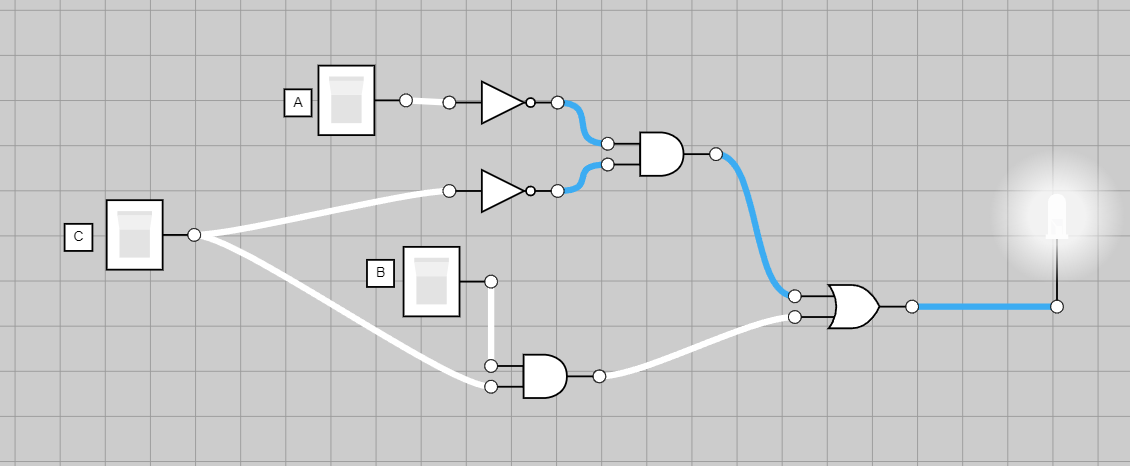
\includegraphics[width=80mm]{circuits/0_0_0.png}\\[0.25in]

            \textbf{0\_1\_0.png is true as seen in the truth table, the LED light is on}\\
            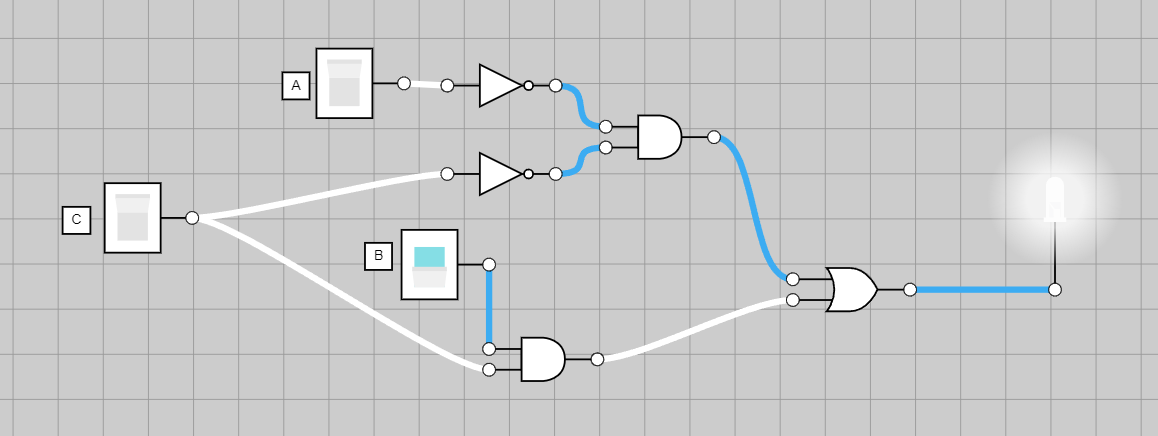
\includegraphics[width=80mm]{circuits/0_1_0.png}\\[0.25in]

            \textbf{0\_1\_1.png is true as seen in the truth table, the LED light is on}\\
            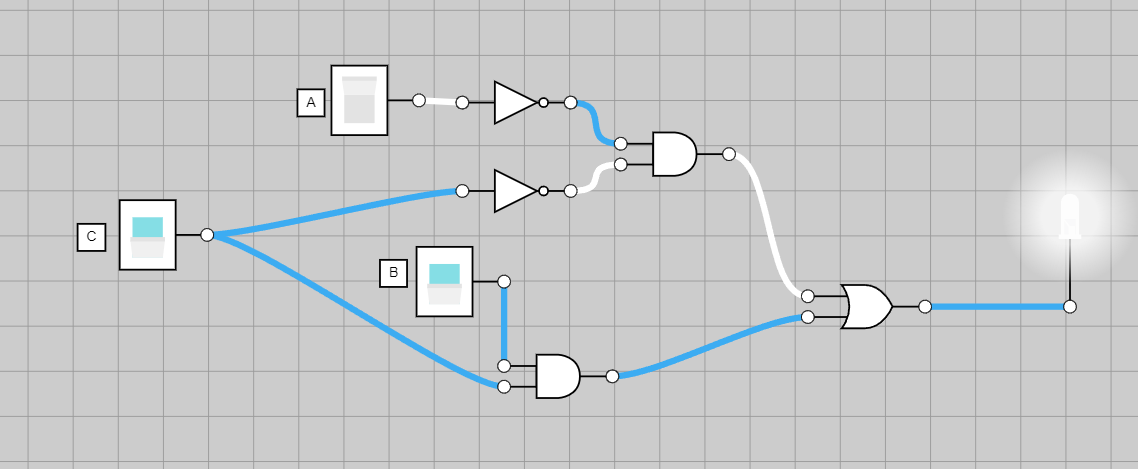
\includegraphics[width=80mm]{circuits/0_1_1.png}\\[0.25in]

            \textbf{1\_1\_1.png is true as seen in the truth table, the LED light is on}\\
            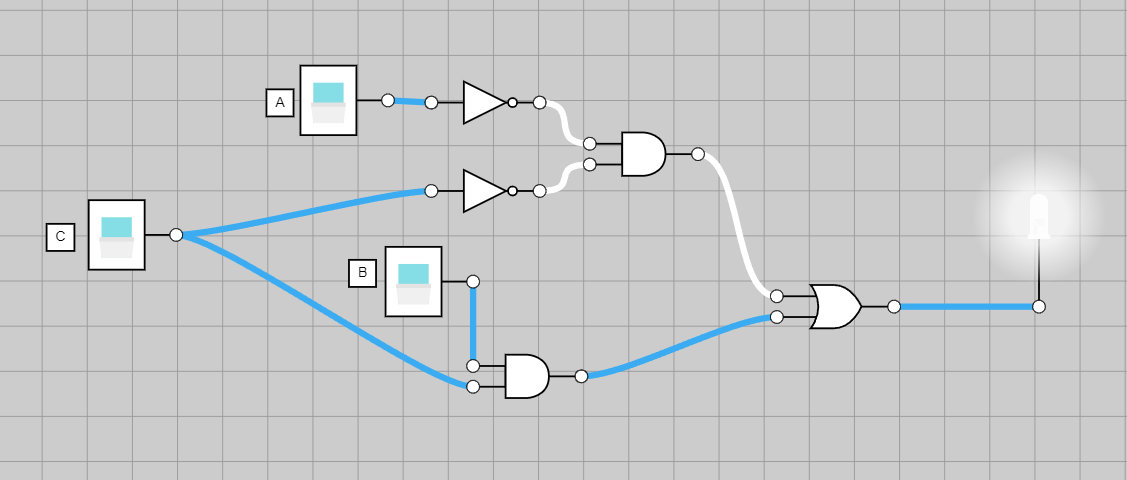
\includegraphics[width=80mm]{circuits/1_1_1.png}\\[0.25in]

            \textbf{0\_0\_1.png is false as seen in the truth table, the LED light is off}\\
            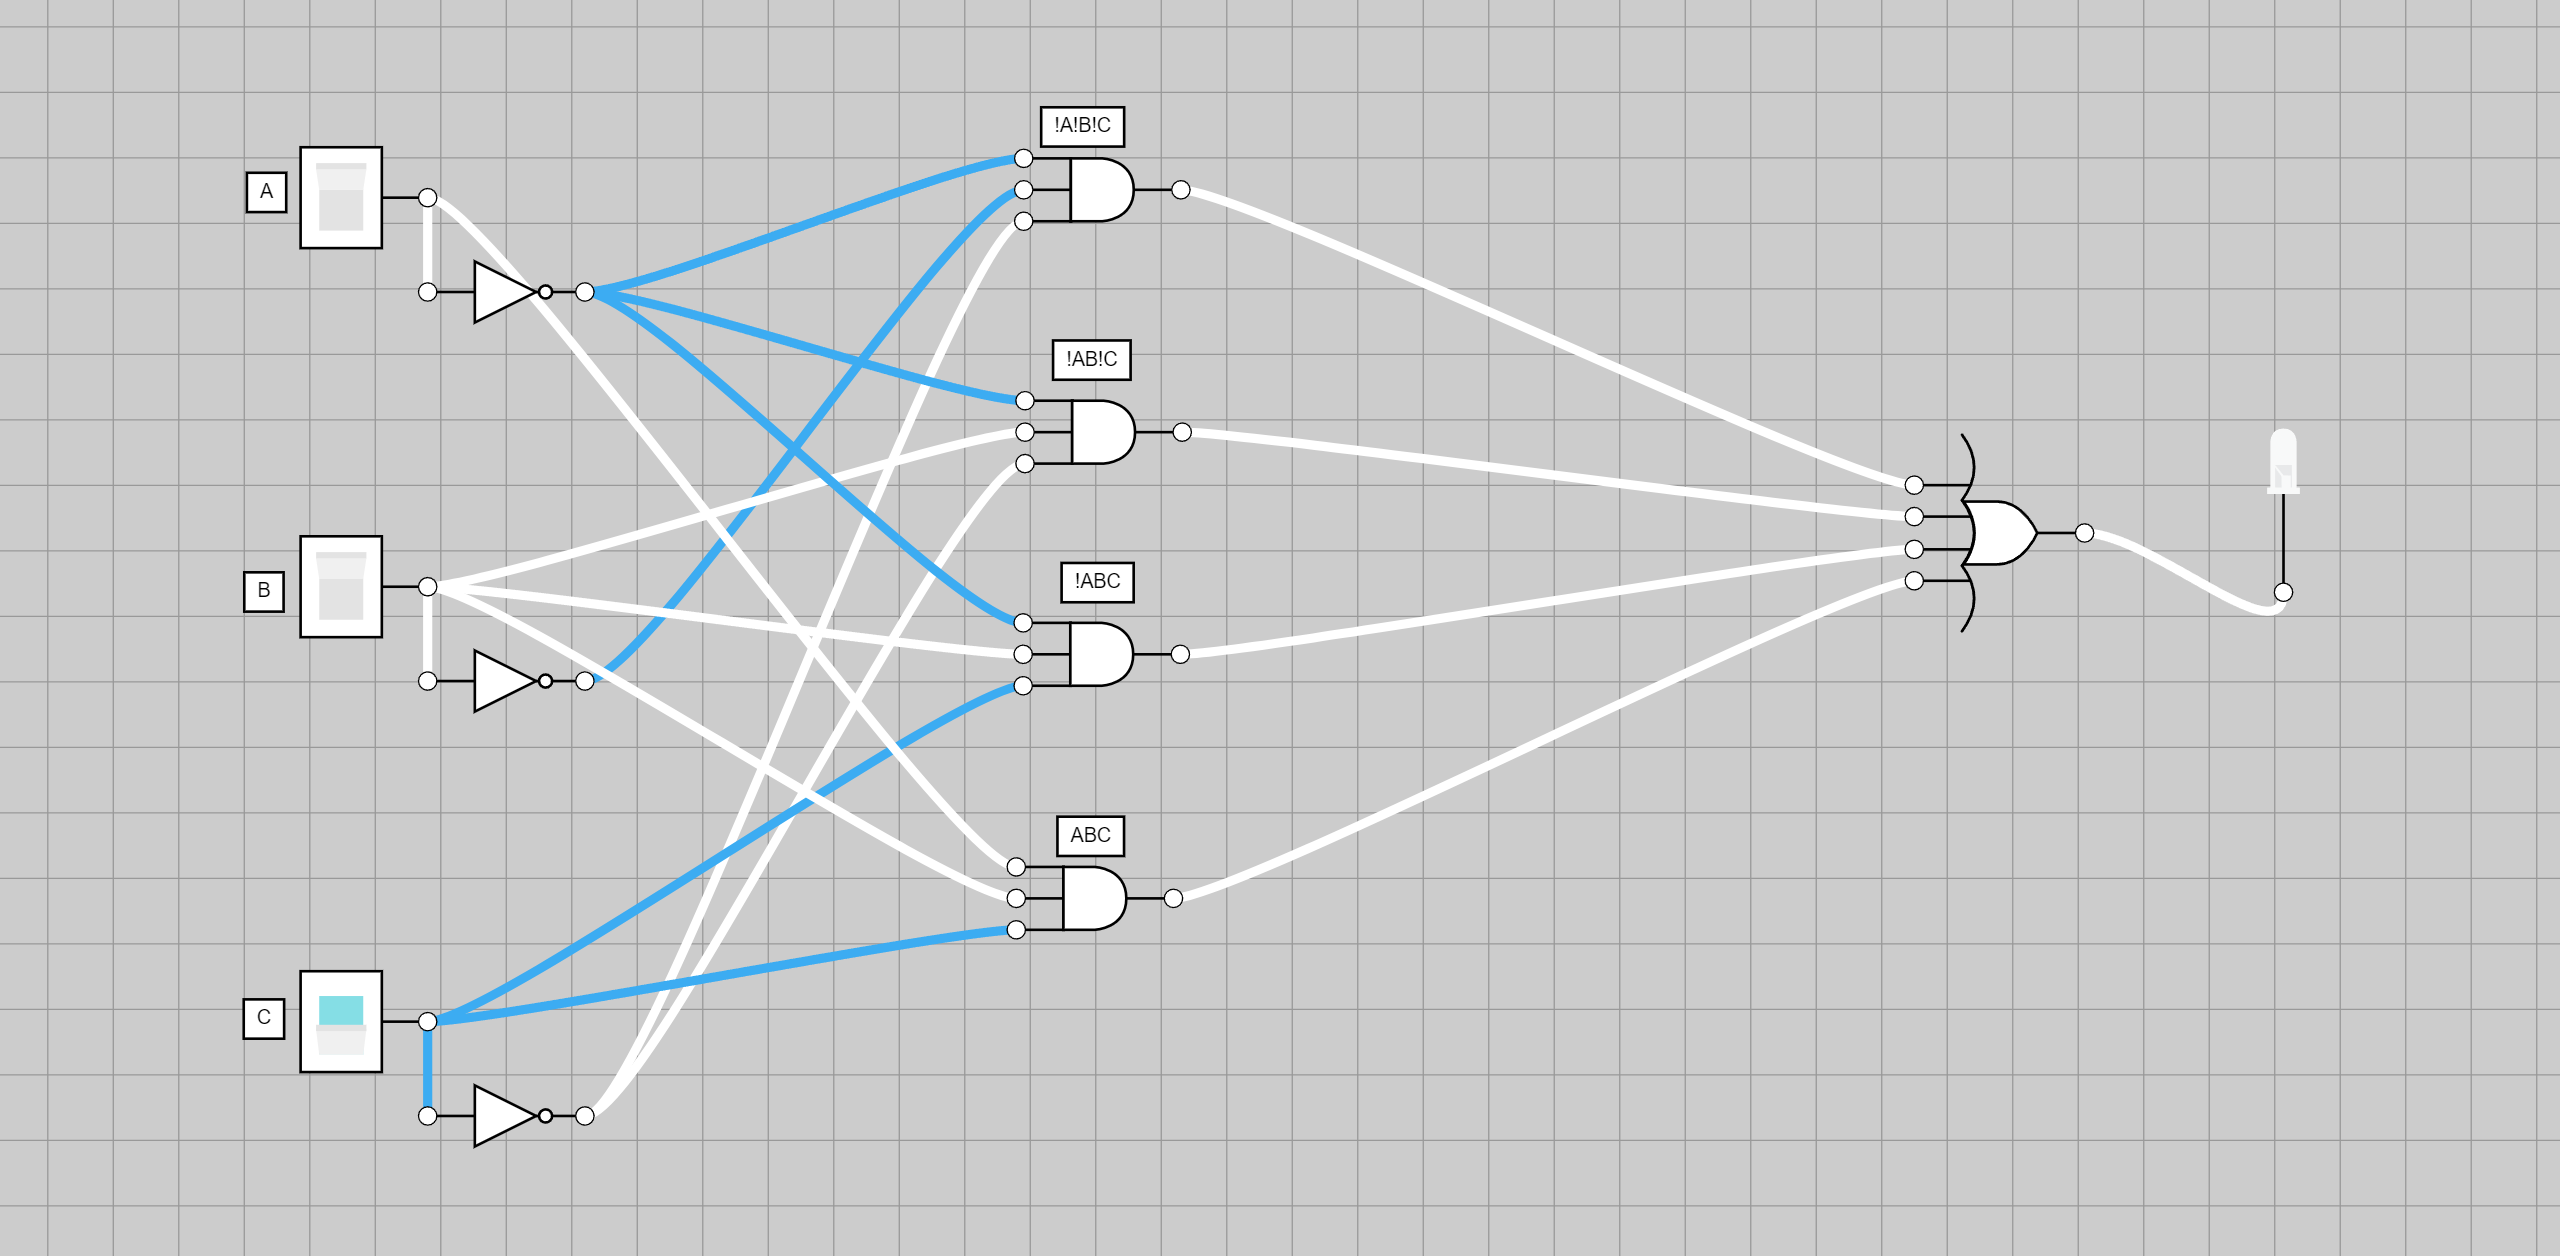
\includegraphics[width=80mm]{circuits/0_0_1.png}\\[0.25in]

            \textbf{1\_0\_0.png is false as seen in the truth table, the LED light is off}\\
            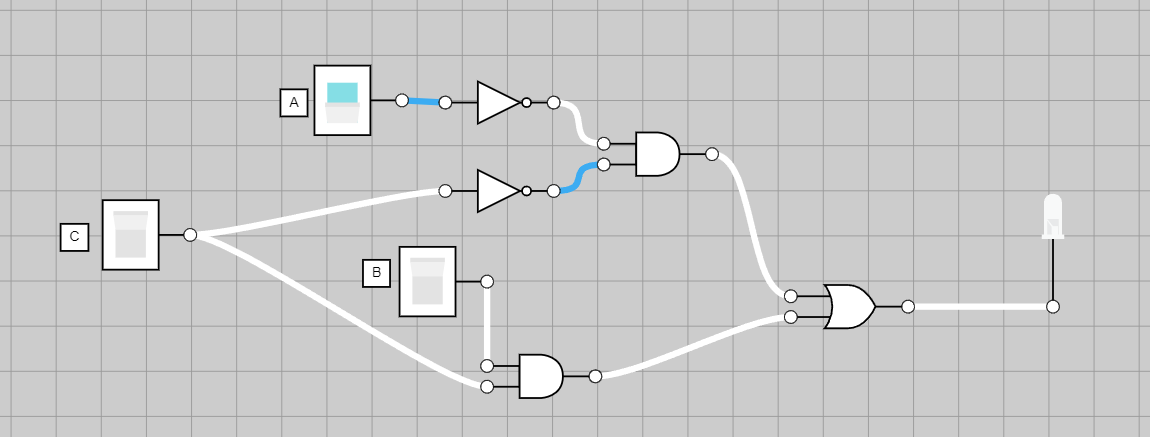
\includegraphics[width=80mm]{circuits/1_0_0.png}\\[0.25in]

            \textbf{1\_0\_1.png is false as seen in the truth table, the LED light is off}\\
            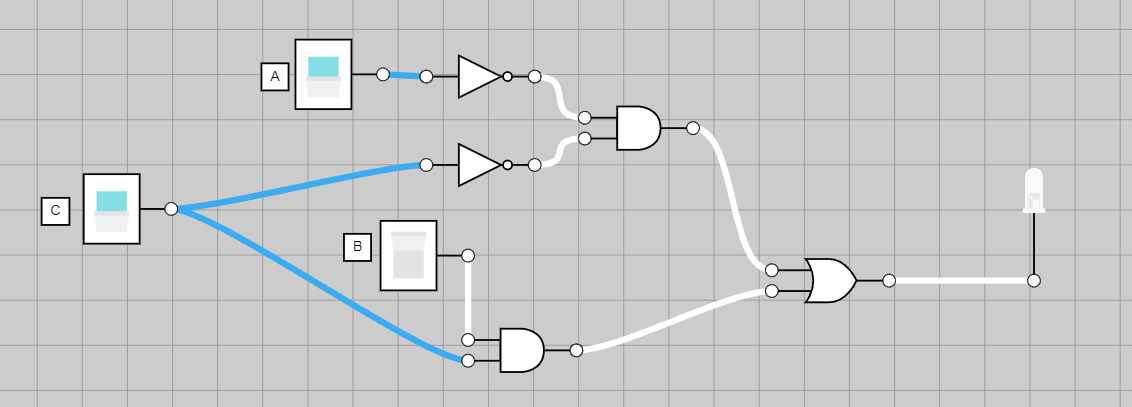
\includegraphics[width=80mm]{circuits/1_0_1.png}\\[0.25in]

            \textbf{1\_1\_0.png is false as seen in the truth table, the LED light is off}\\
            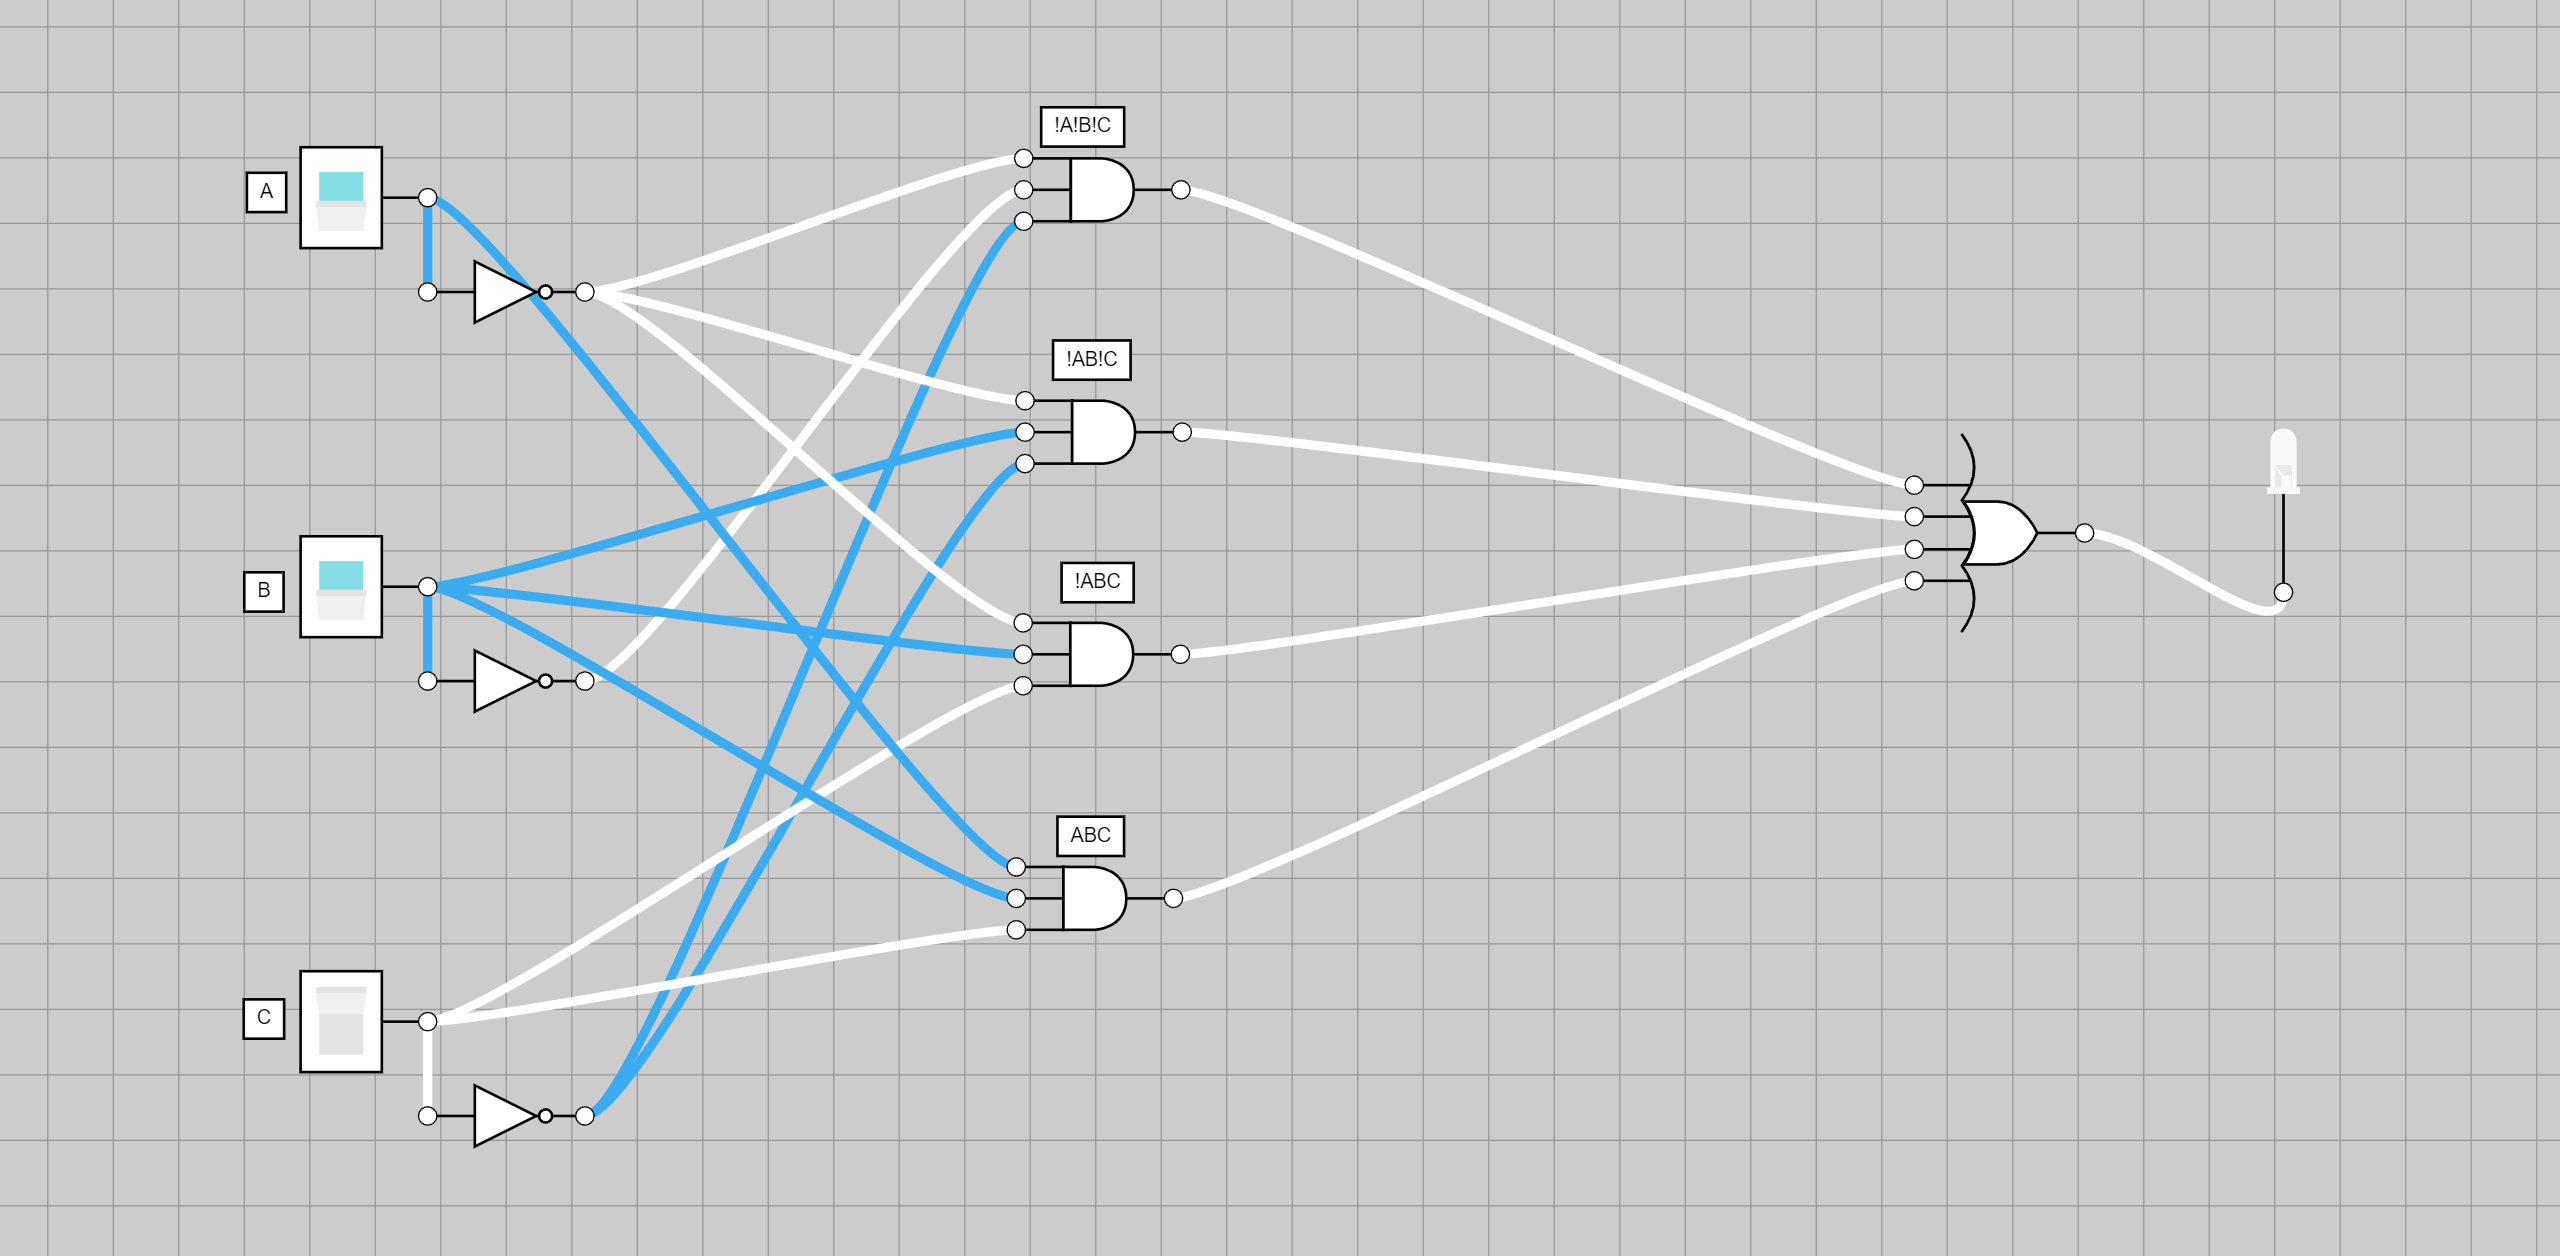
\includegraphics[width=80mm]{circuits/1_1_0.png}\\[0.25in]
        \end{center}
        \item Given inputs A and B, show that NOR {(A + B)} is functionally complete by giving logical
        circuits equivalent to AND {(A * B)}, OR {(A + B)}, and NOT {A} gates using only NOR
        gates in their construction.
        \begin{center}
            \textbf{NOR\_and.circuit represents AND}\\
            \textbf{NOR\_or.circuit represents OR}\\
            \textbf{NOR\_not.circuit represents NOT}
        \end{center}
        \item What is 5ED4 - 07A4 when these values represent unsigned 16-bit hexadecimal numbers? The result should be written in hexadecimal. Show your work.
        \begin{center}
            \begin{tabular}{c c c c c}
                    & $5$ & $E(14)$ & $D(13)$ & $4$\\
                $-$ & $0$ & $7$ & $A(10)$ & $4$\\
                \hline
                & $5$ & $7$ & $3$ & $0$\\
            \end{tabular}\\[0.25in]
            \boxed{\textbf{\LARGE Answer: 5730}}
        \end{center}

        \item What is 5ED4 - 07A4 when these values represent signed 16-bit hexadecimal numbers stored in sign-magnitude format? The result should be written in hexadecimal. Show your work.
        \begin{center}
            \begin{tabular}{c c c c c}
                    & $5$ & $E(14)$ & $D(13)$ & $4$\\
                $-$ & $0$ & $7$ & $A(10)$ & $4$\\
                \hline
                & $5$ & $7$ & $3$ & $0$\\
            \end{tabular}\\[0.25in]
            \boxed{\textbf{\LARGE Answer: 5730}}
        \end{center}

        \textbf{Explanation:}\\
        In sign magnitude, the most significant bit is the sign bit. In our given equations, none of the leading bits are 1: $5 = 0101$, $0 = 0000$, The answer to this problem will be the same as the one prior.

        \item Assume 185 and 122 are unsigned 8-bit decimal integers. Calculate 185 - 122. Is there overflow, underflow, or neither?
        
        \textbf{Decimal to binary conversion}
        \begin{verbatim}
            185 = 1011 1001
            122 = 0111 1010
        \end{verbatim}

        To perform the binary subtraction, we must convert the number being subtracted to a negative binary number using two's complement, and perform binary addition

        \textbf{Find 122 Two's Complement Number}
        \begin{verbatim}
            122 = 0111 1010
                = 1000 0101 <- one's complement (flip all 1's and 0's)
                = 1000 0110 <- add 1 to the end (carried over)
        \end{verbatim}

        \textbf{Calculate 185 + 122(Two's Complement Number)}
        \begin{verbatim}
              1 0000 0000 (carry)
                1011 1001 (185)
            +   1000 0110 (122's Two's Complement Number)
            -------------
              1 0011 1111
        \end{verbatim}

        \textbf{The answer is represented in 9 bits, results in an: }
        \boxed{\text{\LARGE \textbf{OVERFLOW}}}

        \item Assume 151 and 214 are signed 8-bit decimal integers stored in two's complement format. Calculate 151 - 214 using saturating arithmetic. The result should be written in decimal. Show your work.
        
        \textbf{Decimal to binary conversion}
        \begin{verbatim}
            151 = 1001 0111
            214 = 1101 0110
        \end{verbatim}

        \textbf{151 in Two's Complement to obtain original value}
        \begin{verbatim}
                0000 0000 (carry)
                0110 1000 (flip 1's and 0's)
            +           1 (add 1)
            -------------
                0110 1001
        \end{verbatim}

        \textbf{214 in Two's Complement to obtain original value}
        \begin{verbatim}
                0000 0010 (carry)
                0010 1001 (flip 1's and 0's)
            +           1 (add 1)
            -------------
                0010 1010
        \end{verbatim}

        \textbf{Convert numbers back to decimal}
        \begin{verbatim}
            (151) 0110 1001 = 105
            (214) 0010 1010 = 42
        \end{verbatim}

        \textbf{Perform operation}\\[0.25in]
        105 - 42 = \boxed{\text{\LARGE \textbf{63}}}\\[0.25in]
        For 8-bit signed integers, saturation limits are from $-128$ to $127$, since $-128\leq63\leq127$, no saturation is required.

        \item Assume 151 and 214 are unsigned 8-bit integers. Calculate 151 + 214 using saturating arithmetic. The result should be written in decimal. Show your work.
        
        \textbf{Simple Addition}
        \begin{verbatim}
            151 + 214 = 365
        \end{verbatim}

        \textbf{Saturation}\\
        For 8 bit unsigned integers, saturation limits are from 0 to 255, since $365 > 255$, the final answer will be saturated to the bounds of 255.

        151 + 214 = \boxed{\text{\LARGE \textbf{255}}}

        \item What decimal number does the bit pattern 0×0C000000 represent if it is a two's complement integer? An unsigned integer?
        \begin{verbatim}
            0x0C000000 = 
            0000 1100 0000 0000 0000 0000 0000 0000
            ^ left most bit is 0, positive integer

            equation becomes 2^27 + 2^26 = 201 326 592
        \end{verbatim}
        \begin{center}
            \boxed{\text{\LARGE \textbf{Two's Complement: $201 326 592$}}}\\
            \boxed{\text{\LARGE \textbf{Unsigned integer: $201 326 592$}}}\\
        \end{center}
        
        \textbf{Since the binary representation's most signifcant bit is a 0, both will have the same value}

        \item If the bit pattern 0×0C000000 is placed into the Instruction Register, what MIPS instruction will be executed
        \begin{verbatim}
            MIPS opcode takes in 6 bits, from the most signifcant onwards
            0000 11 <- opcode
            0000 11 is MIPS's jal instruction
        \end{verbatim}
        \begin{center}
            \boxed{\text{\LARGE \textbf{jal 0}}}\\
        \end{center}
        
        \item Give a reason why we use two’s complement representation for negative numbers in computer
        arithmetic. Give an example of its usage.\\[0.25in]
        \textbf{
            We use Two's Complement representation for negative numbers 
            because it simplifies addition and subtraction with negative 
            numbers easier. To take Two's Complement, you must take One's 
            Complement first, simply take the positive version of the negative 
            number, and flip over all 0's and 1's.
        }
        
        \textbf{
            However, One's Complement works, but for the number 0, it has two
            representation(0000 and 1111), to remove this. We take Two's
            Complement. We take One's Complement of the number, then we add 1
            to the end.
        }\\[0.25in]

        \textbf{Normal signed int}
        \begin{verbatim}
            Assume we want to do 5 + (-5): 
            5 = 0101
           -5 = 1101

           when we perform the addition, we are expecting a 0, right...?
           
                                1010 (carry)
                       5        0101
                    + -5    +   1101
                    ----    --------
                    0          10010
            
    we get a value of 10010, getting rid of overflow, we get 0010, but 0010 = 2?
        \end{verbatim}

        \textbf{Two's Complement}
        \begin{verbatim}
            

        Using Two's Complement: 
        5 = 0101
        flip 1's and 0's
        5 = 1010
        add 1 to the end
        -5 = 1011

           1110 (carry)
           0101
        +  1011
        -------
          10000

here, we get a value of 10000, getting rid of the overflow, we get 0000, and 0000 = 0.
        \end{verbatim}
    \end{enumerate}
\end{document}